
\section{选题意义与可行性分析}

进入新时代,人和人交流更多了。但是语言仍然是无阻碍交流里不可逾越的鸿沟,为了跨过这个鸿沟,
我们花费了太多代价。无数的书籍、文献亟待翻译。人力资源不仅短缺,也很昂贵。
无数先锋开发出了多种数学模型试图翻译,很多确实在工作的特别好。但是,要用一个数学模型去做翻译,缺点太多。
语言不是简单的能用公式就表达的清楚的。不是简单的用一个数学模型去隐射就能翻译的。
要正确的进行翻译,源文本的意思必须要被理解。

\begin{wrapfigure}{8}{12em}%
\begin{center}%
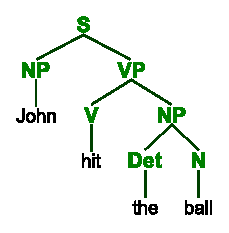
\includegraphics{../ParseTree}%
\\\textbf{一个简单的语法树}%
\end{center}%
\end{wrapfigure}%
举一个简单的例子来说吧。
这一方面编译器就做的很到位。高级语言本身已经很接近人类语言了,
编译器依然能够理解并翻译成机器语言。
这种翻译是一种精确的翻译。人类的言语可以使用这样的模型翻译么?

\nocite{Compilers_Principles_Techniques_and_Tools}


理解?如何让计算机理解文字?答案是语法树\cite{cst}。语法树是计算机程序使用
的单根有序树形数据结构。语法树使用BNF\cite{BNF}声明进行描述。

\framedparbox{
%\fbox{
\vspace*{2ex}
 <symbol> ::= \_\_expression\_\_ 
\vspace*{2ex}
 }
 
 这里的 <符号> 是非终结符,而表达式由一个符号序列,或用指示选择的竖杠 `|' 分隔的多个符号序列构成,每个符号序列整体都是左端的符号的一种可能的替代。从未在左端出现的符号叫做终结符。 
 对于句子 \fbox{\tt John hit the ball}. 这里给出了一个不太完整的用于分析此句子的BNF声明 \\

\fbox{\begin{minipage}{12cm}
% \framedparbox{
%\fbox{\vbox{
\vspace*{2ex}
ENDPUNC ::= '.' | '?' 

S ::= NP VP ENDPUNC | NP ENDPUNC | VP ENDPUNC | ...  < more >

NP ::= Det N | N  | Pron | < more >

Det ::= "the" | "an" | "a" | "this" | ... ...  < more >

V ::= "hit" | ...... < more >

N ::= "ball" | .... < more >

Pron ::= I | "you" | ..... <more>

.... <more>

\vspace*{2ex}
\end{minipage} }


可见,至少此简单的英文句子是可以被BNF文法声明的。英语句型就那么几个,复杂的句子都是组合而成的。而BNF
提供了对递归定义的良好支持。这就在理论上提供了分析任意英文句法的可行性。

而 BNF 声明进一步扩展,这是 Bison\cite{bison} 语法描述文件的基础。Bison 通过读取语法描述文件,可以
自动构建出能特定解析语法的解析程序。

\section{研究的基本内容与拟解决的主要问题}

而要做到构建语法树,需要2个前提条件,有了这个,Bison 才可以构建出语法树生成程序。这2个条件就是
\begin{enumerate}
\item 单词扫描程序。单词扫描程序将源语句分段,分拆成一个一个单词和标点。
\item 词性标记程序。向语法解析程序传递非常重要的讯息:词性。而这个正是 BNF 声明中 NP 中的 N。词性标记程序标记好词性,比如标记为 N ,才能在依据后续输入 NP VP 等这些句型中做选择。
\end{enumerate}

单词扫描程序非常简单,就是用一系列的正则表达式去匹配字符串,英语中单词之间都是用空格分隔的,所以甚至都不需要复杂的正则表达式去匹配,简单的依据空格或标点分隔就已经能很好的工作了。

词性标记程序。主要是利用词典决定词性。但是对于多词性单词,无法直接判断词性。这时可以使用 HMM\cite{HMM_Based_Part_Of_Speech_Tagging} 来标记词性。 HMM 是 ANN(人工神经网络)的一种。
主要解决对确定的观察符号到不确定的隐藏符号的隐射。一个句子的每个单词是一个观察符号,而单词对应的词性是隐藏符号。
每个单词可能对应的词性是非常不确定的,但是一个具体的句子中,又是特定的。程序执行的一开始,首先由字典来过滤掉大部分的结果,如果还有单词无法确定词性,就进入 HMM 状态。HMM 是一种神经网络,非常擅长复杂数据之间的隐射。比如一幅图像到一个人名的隐射\footnote{对,这就是人脸识别}。一句子中,每个单词的词性必定是唯一对应的。这个对应可以先通过训练教会 HMM, 此后 HMM 就可以触类旁通地自动掌握类似句子的匹配。

\section{总体研究思路及预期研究成果}

研究前人对于标记词性的经验和成果,特别是基于 HMM 的词性标记。被标记了词性的单词序列就可以进入下一步
语法树生成步骤。为英语语言定义一种能描述它的语法树。如此一来,计算机就能初步算是理解了英语这个自然语言。
此研究成锅后续可以用到自然语言处理、机器聊天程序、以及自动翻译。

预期做出一个Demo完成语法树生成。

\section{研究工作计划}

年底前拜读机器翻译大师的作品,找到一些前人已经有的功能,避免重复发明轮子。
次年开始构筑翻译Demo
次年3月完成Demo和论文。


\section{参考文献}

\nocite{STATMT}
\bibliography{../reference}
\bibliographystyle{plain}
